\pagestyle{plain}
\graphicspath{{Chapter2/Figs/Raster/}{Chapter2/Figs/}}
% \chapter{Mô hình Boosted Tree}
\chapter{MÔ HÌNH BOOSTED TREE}
Trong chương này, đồ án giới thiệu về phương pháp học máy có giám sát, tổng quan về phương pháp học Ensemble Learning và một mô hình cụ thể của phương pháp này là Boosted Tree.
\section{Học có giám sát - Supervised Learning}
\subsection{Giới thiệu}
Học có giám sát (Supervised learning) là thuật toán dự đoán đầu ra (outcome) của một dữ liệu mới (new input) dựa trên các cặp (input, outcome) đã biết từ trước. Cặp dữ liệu này còn được gọi là (data, label), tức (dữ liệu, nhãn). Supervised learning là nhóm phổ biến nhất trong các thuật toán Machine Learning.

Một cách tổng quát, khi chúng ta có một tập hợp các biến đầu vào \( \mathcal{X} = \{\mathbf{x}_1, \mathbf{x}_2, \dots, \mathbf{x}_N\} \) và một tập hợp nhãn tương ứng \( \mathcal{Y} = \{\mathbf{y}_1, \mathbf{y}_2, \dots, \mathbf{y}_N\} \), trong đó \( \mathbf{x}_i, \mathbf{y}_i \) là các vector. 
Các cặp dữ liệu biết trước \( (\mathbf{x}_i, \mathbf{y}_i) \in \mathcal{X} \times \mathcal{Y} \) được gọi là tập training data (dữ liệu huấn luyện). Từ tập traing data này, chúng ta cần tạo ra một hàm số ánh xạ mỗi phần tử từ tập \(\mathcal{X}\) sang một phần tử (xấp xỉ) tương ứng của tập \(\mathcal{Y}\):

\[ \mathbf{y}_i \approx f(\mathbf{x}_i), ~~ \forall i = 1, 2, \dots, N\] Mục đích là xấp xỉ hàm số \(f\) thật tốt để khi có một dữ liệu \(\mathbf{x}\) mới, chúng ta có thể tính được nhãn tương ứng của nó \( \mathbf{y} = f(\mathbf{x}) \). \\
\begin{figure}[H]
    \centering
    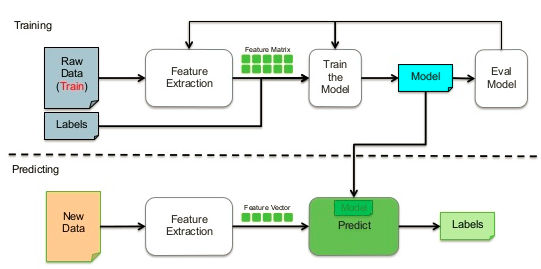
\includegraphics[scale=1.0]{supervised-learning}
    \caption{Mô hình hoạt động của Học có giám sát}
    \label{fig:my_labe3}
\end{figure}
\indent Bài toán Supervised learning còn được chia thành 2 bài toán chính: 
\begin{itemize}
\ii \textbf{Phân loại - Classification}: các label của input data được chia thành một số hữu hạn nhóm. Ví dụ: Dự đoán kiểu tấn công dựa vào một luồng traffic cho trước. Dự đoán một tin nhắn là spam hay không, ...\\
\ii \textbf{Hồi quy - Regression}: Các label không được chia thành nhóm mà có 1 giá trị cụ thể. Ví dụ: Ước lượng giá của một căn nhà dựa trên diện tích.
\end{itemize}
Với mô hình hồi quy tuyến tính, $\hat{y}$ được tính bằng:\\
\begin{equation}
    \hat{y_i}= \sum_{j} \theta_j x_{ij}
\end{equation}
Ta có $\hat{y_i}$ là giá trị dự đoán được dựa trên input $x$ và trọng số $\theta$ - thành phần cần được học dựa trên bộ training data. 

\subsection{Hàm mục tiêu}

Dựa vào các cách hiểu và sử dụng $y_i$ khác nhau, các mô hình khác nhau được ra đời: phân loại, hồi quy, ... Khi huấn luyện một mô hình học có giám sát,  tập dữ liệu (dataset) được chia làm 2 phần: \textit{tập huấn luyện} (training set) và \textit{tập kiểm thử} (testing set).
\begin{itemize}
\ii  \textbf{Tập huấn luyện}: được sử dụng để học - tức quá trình tối ưu hóa tham số $\Theta$, xây dựng mô hình.
\ii \textbf{Tập kiểm thử}: được sử dụng để đánh giá độ tốt của mô hình. Dữ liệu test được giả sử là không được biết trước, và không được sử dụng để xây dựng các mô hình Machine Learning.
\end{itemize}
\indent Huấn luyện mô hình là quá trình tìm một phương pháp huấn luyện trên tập huấn luyện sao cho mô hình dự đoán tốt trên tập kiểm thử. Người ta thường ít quan tâm đến độ tốt của mô hình trên tập huấn luyện bởi vì nó thường rất cao. Độ tốt trên tập huấn luyện chỉ thể hiện được \textbf{khả năng ghi nhớ} của mô hình về những gì đã nhìn thấy. Với một mô hình tốt thật sự, ta cần thêm \textbf{khả năng tổng quát hóa}, chính là việc dự đoán tốt trên dữ liệu chưa hề được nhìn thấy. \\
\indent Để làm được 2 điều trên, hàm mục tiêu được sử dụng trong quá trình học. Hàm mục tiêu được định nghĩa bởi công thức sau:
\begin{equation}
    Obj(\Theta) = L(\Theta) + \Omega(\Theta)
\end{equation}
Với $L$ được gọi là \textit{hàm mất mát huấn luyện} (training loss function) và $\Omega$ được gọi là \textit{hàm chuẩn tắc} (regualarization). Hàm mất mát phản ánh độ tốt của mô hình trên tập huấn luyện. $L$ được tính bởi công thức:
\begin{equation}
    L = \sum_{i=1}^{n} l(y_i,\hat{y_i})
\end{equation}
 Hàm mất mát phổ biến thường được sử dụng là mean squared error:
\begin{equation}
l(y_i, \hat{y_i}) = (y_i - \hat{y_i})^2
\end{equation}
Một hàm mất mát phổ biến khác sử dụng trong phương pháp logistic regression là:
\begin{equation}
l(y_i, \hat{y_i}) =  y_i\ln (1+e^{-\hat{y}_i}) + (1-y_i)\ln (1+e^{\hat{y}_i})
\end{equation}

$L$ càng nhỏ có nghĩa mô hình càng \textit{khớp} với tập huấn luyện. Tuy nhiên, trong thực tế, việc một mô hình quá \textit{khớp} với dữ liệu sẽ bị phản tác dụng. Việc quá khớp này có thể dẫn đến việc dự đoán nhầm nhiễu, và chất lượng mô hình không còn tốt trên dữ liệu kiểm thử nữa. Mô hình trở nên quá phức tạp để mô phỏng dữ liệu huấn luyện. Điều này đặc biệt xảy ra khi lượng dữ liệu huấn luyện quá nhỏ trong khi độ phức tạp của mô hình quá cao. Hiện tượng này gọi là \textit{quá khớp} (overfitting). \\

\indent Hàm regularization được sinh ra để giải quyết vấn đề này. Regularization, một cách cơ bản, là thay đổi mô hình để tránh quá khớp trong khi vẫn giữ được tính tổng quát của nó (tính tổng quát là tính mô tả được nhiều dữ liệu, trong cả tập huấn luyện và kiểm thử). Điều này làm cho mô hình \textit{đơn giản hơn} mặc dù giá trị của hàm mất mát có tăng lên. Tuy nhiên nếu regularization quá lớn sẽ làm mô hình xảy ra hiện tượng \textit{không kxhớp} (underfitting). Ngược lại với quá khớp, underfitting sẽ khiến khả năng dự đoán của mô hình trên tập huấn luyện giảm.\\


\begin{figure}[H]
  \centering
  \begin{subfigure}
    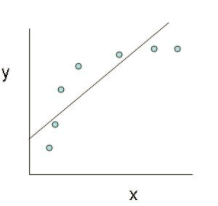
\includegraphics[scale=1.0]{underfit}
    \subcaption{underfit}
    \label{fig:f1}
  \end{subfigure}
  \begin{subfigure}
    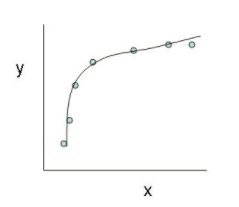
\includegraphics[scale=1.0]{good}
    \subcaption{good}
    \label{fig:f2}
  \end{subfigure}
  \begin{subfigure}
    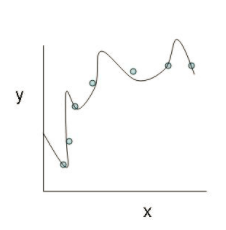
\includegraphics[scale=1.0]{overfit}
    \subcaption{overfit}
    \label{fig:f3}
  \end{subfigure}
  \caption{Ví dụ minh họa về overfit và underfit}
\end{figure}



Như vậy, hàm mục tiêu sẽ giúp mô hình đáp ứng được tính dự đoán cao và tính đơn giản. Việc làm này còn được gọi là bias-variance tradeoff\cite{tradeoff}.
\section{Ensemble Learning}
\subsection{Giới thiệu}
Trong thực tế, dữ liệu thu thập được từ nhiều nguồn có thể khác nhau về bản chất. Một phân loại được tạo ra từ một thuật toán học có thể đạt được độ chính xác cao với một số bộ dữ liệu này nhưng lại có tỉ lệ sai cao hơn trong một số bộ dữ liệu khác. Cụ thể, việc áp dụng các thuật toán học khác nhau vào một tập dữ liệu có thể tạo ra kết quả phân loại khác nhau. Không có thuật toán học đơn lẻ nào thực hiện tốt trên tất cả các bộ dữ liệu. Thực nghiệm cho thấy các thuật toán đơn giản như K-neighbour neighbor (kNN) trong một số trường hợp có thể có độ chính xác cao hơn so với các phương pháp phức tạp hơn như Decision Tree hoặc Support Vector Machine (SVM). 
\\Một cách tiếp cận khác để thu được hiệu suất cao trong việc phân loại là kết hợp nhiều thuật toán học với nhau để có được độ chính xác cao hơn so với một thuật toán duy nhất. Nhìn chung, rất khó để biết một thuật toán học nào phù hợp cho một tập dữ liệu cụ thể. Phương pháp Ensemble kết hợp các mô hình khác nhau với mục tiêu đạt được tỷ lệ lỗi phân loại thấp hơn so với sử dụng một mô hình duy nhất. Khái niệm "mô hình" trong các phương pháp kết hợp được hiểu theo nghĩa rộng, bao gồm không chỉ việc thực hiện các thuật toán học khác nhau, hoặc tạo ra nhiều tập huấn luyện cho cùng một thuật toán học, mà còn là sinh ra các bộ phân loại chung kết hợp với nhau để nâng cao độ chính xác phân loại.
\subsection{Cách thức hoạt động}
Giả sử có N quan sát. Một thuật toán học có đầu ra là một bộ phân loại là một hàm hypothesis thể hiện quan hệ $f$ giữa các quan sát và các nhãn. Nhãn của quan sát \textbf{$x$} sẽ được dự đoán dựa trên hypothesis. Một hệ thống gồm $K$ thuật toán học sẽ cho ra $K$ hàm hypothesis, ký hiệu bởi $h_1, h_2, ..., h_k$. Dietterich[7] đã cho thấy 3 lý do vì sao một phương pháp ensemble lại tốt hơn một bộ phân loại đơn lẻ. (Hình 2.3)
\begin{figure}[H]
    \centering
    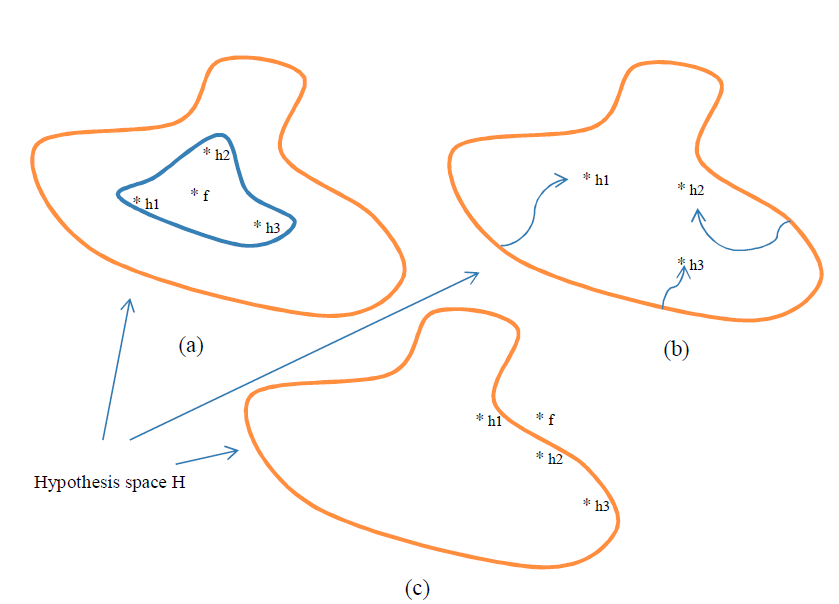
\includegraphics[scale = 0.7]{Chapter2/Figs/hypothesis.PNG}
    
    \centering
    \caption{Ba lý do phương pháp Ensemble tốt hơn}
    \label{fig:my_label}
\end{figure}


\begin{enumerate}[label=(\alph*)]
\item Tính thống kê (Statistical): Trong một số trường hợp, số lượng quan sát trong một tập huấn luyện là không đủ so với kích thước của không gian hypothesis H bao gồm tất cả các hypothesis được tạo ra bởi một thuật toán học. Do đó, thuật toán sẽ tìm kiếm trên nhiều hypothesis có cùng tỷ lệ lỗi. Bằng cách sử dụng phương pháp emsemble, chúng ta có thể thực hiện bình chọn bình chọn trong số tất cả các thuật toán học. 
\item Khả năng tính toán (Computational): Rất nhiều thuật toán sử dụng phương pháp tìm kiếm cục bộ để thu được giải pháp tối ưu cục bộ. Trong phương pháp ensemble, bằng cách thay đổi điểm bắt đầu (starting point) của các thuật toán học, chúng ta có thể thu được một hàm xấp xỉ tốt hơn thể hiện quan hệ  $f$ giữa vector đặc trưng \textbf{$x$} và nhãn \textbf{$y_x$} so với một thuật toán đơn lẻ. 
\item Tính đại diện (Representational): Quan hệ $f_x$ giữa \textbf{$x$} và  \textbf{$y_x$} trong một vài trường hợp không thể mô hình hóa bởi một hypothesis đơn. Với phương pháp ensemble, điều này có thể giải quyết bằng cách kết hợp nhiều hypothesis lại. 
\end{enumerate}
% \section{Một số phương pháp Ensemble Learning}
% \subsection{Các phương pháp họ Bagging}
% Bagging là viết tắt của "Boostrap Aggregating", được giới thiệu bởi Breiman[8]. Cách tiếp cận này tạo ra tập huấn luyện mới từ nguyên bản bằng cách sử dụng phương thức bootstrap trong thống kê. Trong kỹ thuật này, các quan sát được rút ra và được thay thế từ tập huấn luyện cho đến khi kích thước của tập huấn luyện mới bằng kích thước của tập đầu. Các quan sát có thể xuất hiện nhiều lần trong tập mới. Kết quả của quá trình lấy mẫu lại này là tập huấn luyện mới không độc lập thống kê so với tập huấn ban đầu, mặc dù sự đa dạng đạt được bằng cách có nhiều chương trình tập huấn. Một thuật toán học chạy trên tất cả các tập huấn luyện được tạo ra, và đầu ra được kết hợp theo một cách nào đó, chẳng hạn như bỏ phiếu.\\
% \indent Bagging yêu cầu các thuật toán học không ổn định. Điều này đồng nghĩa với việc chỉ cần dữ liệu học thay đổi ít thì thuật toán học sẽ sinh ra một bộ phân loại khác. Với cách tiếp cận bagging, tập huấn luyện mới tượng tạo ra dựa trên việc thay thế ngẫu nhiên, $1/e \approx 36.8\%$ các quan sát ban đầu trong tập huấn luyện sẽ không xuất hiện trong tập mới[9]. Các quan sát được chọn với xác suất như nhau. Nếu thuật toán học ổn định, đầu ra của thuật toán là các bộ phân loại với sự khác biệt rất ít. Kết quả là khi kết hợp các bộ phân loại này sẽ được một mô hình gần giống với việc chỉ dùng một bộ phân loại đơn lẻ. Vì lý do này, chỉ các thuật toán bất ổn định như Cây quyết định - Decision Tree (DT) và mạng Neural được sử dụng trong Bagging. 
% \begin{figure}[H]
%     \centering
%     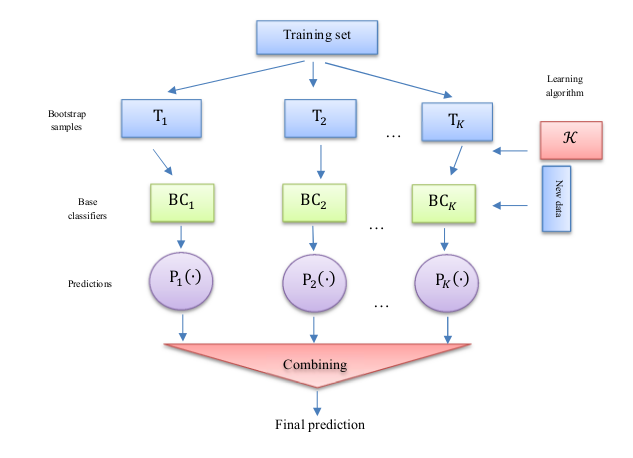
\includegraphics[scale=0.8]{Chapter2/Figs/bagging.png}
%     \caption{Mô hình Bagging}
%     \label{fig:my_label12312}
% \end{figure}
% \subsection{Các phương pháp họ Boosting}
\section{Boosting}

\begin{figure}[H]
    \centering
    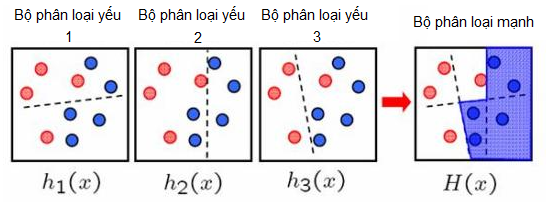
\includegraphics{Chapter2/Figs/weak-learner.PNG}
    \caption{Boosting}
    \label{fig:my_label}
\end{figure}
Phương pháp ensemble learning nổi tiêng nhất là Boosting, phương pháp mà Breiman \cite{16} cho rằng có quan trọng nhất trong việc phân loại trong thế kỷ 20. \\
\indent Ý tưởng của cách tiếp cận này là kết hợp các giải thuật học yếu (weak learner), có độ chính xác lớn hơn 50\%, tức là lớn hơn đoán ngẫu nhiên, nhằm đạt được tỷ lệ lỗi thấp hơn các thuật toán học yếu chạy trên cùng tập huấn luyện (xem Algorithm 1). 

\begin{algorithm}
 \caption{Thủ tục chung cho các phương pháp Boosting}
 \label{algo_1}
 \begin{algorithmic}[1]
 \renewcommand{\algorithmicrequire}{\textbf{Input:}}
 \renewcommand{\algorithmicensure}{\textbf{Output:}}
\REQUIRE Dataset $D$\\
        Thuật toán học $K$\\
        Số lần lặp $M$ \\
        
% \ENSURE  Optimal value of $\alpha$ and base classifiers $BC_k$ ($k=1,\ldots ,K$)
%  \textit{(Khởi tạo bộ phân loại cơ sở)}
\STATE Khởi tạo $D_1 = D$ 
\FOR{$m = 1\ldots M$}
    \STATE Học hypothesis $h_m = Learn(K, D_m)$;
    \STATE Tính error rate $e_m = P_{x ~ D_m}(h_m(x) \neq y_x)$\\
    $D_{t+1} = Adjust\_distribution(D_m, e_m)$
\ENDFOR
\ENSURE $H = Combine\_outputs(h_1, h_2, ..., h_M)$
\end{algorithmic} 
\end{algorithm}

\section{Boosted Tree}
Là một phương pháp Boosting, Boosted Tree xuất phát từ ý tưởng kết hợp các mô hình cây phân loại để tạo ra một mô hình mới tốt hơn.


\subsection{Mô hình cây - Tree model}
Một mô hình cây là một cấu trúc dữ liệu gồm các nút (node) liên kết với nhau. Nút ở trên cùng của cây gọi là gốc (root). Mỗi nút lại gồm nhiều các nhánh con. Nút ở dưới cùng của cây gọi là lá (leaf). Các mô hình cây thường có khả năng dự đoán hạn chế. Nhưng khi kết hợp các mô hình cây lại với nhau như trong Bagged trees (1996), Random Forest (2001) của Breiman \cite{16}, hoặc trong thuật toán Boosted Tree để tạo thành một bộ phân loại mới có khả năng dự đoán tốt hơn. Có nhiều cây \textit{yếu} như Decision Tree (Cây quyết định) , CART (classification and regression trees - Cây phân loại và hồi quy),... \\
Phương pháp Boosted Tree sử dụng các cây CART làm các cây cơ sở. CART có một chút khác biệt so với cây quyết định bình thường, mỗi lá của cây là một giá trị thực. Giá trị này cho chúng ta nhiều diễn giải phong phú hơn so với việc phân loại thông thường. Điều này sẽ làm cho việc tối ưu hóa đơn giản hơn. \\

CART được tạo nên bằng một giải thuật tham lam theo cách tiếp cận từ trên xuống (top-down) sử dụng phân chia nhị phân. Từ gốc, các cách chia nhánh con được đưa ra để chọn lựa, cách chia nhánh nào tối thiểu hóa được hàm mục tiêu sẽ được chọn. Thủ tục này được thực hiện đệ quy cho đến khi thỏa mãn một số tiêu chí dừng.\\ 



\indent Ví dụ dưới đây sử dụng 2 cây để phân loại các thành viên gia đình vào các lá khác nhau và gán các giá trị cho mỗi lá. Điểm của mỗi thành viên trong gia đình được tính bằng tổng điểm thu được ở mỗi cây.
\begin{figure}[H]
    \centering
    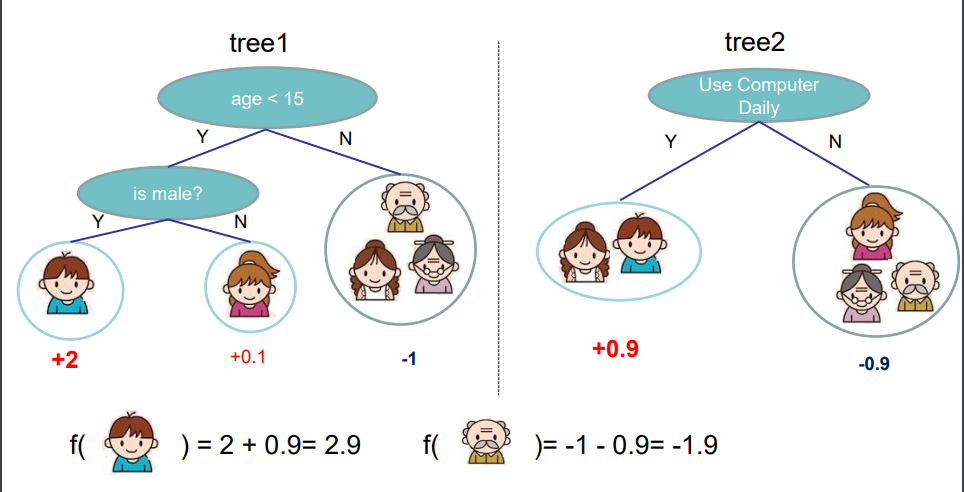
\includegraphics[scale=0.5]{Chapter2/Figs/tree_example.PNG}
    \caption{Ví dụ minh họa về  Boosted Tree}
    \label{fig:my_label}
\end{figure}
Việc tính điểm có thể tổng quát hóa thành:
\begin{equation}
    \hat{y}_i = \sum_{k=1}^K f_k(x_i), f_k \in \mathcal{F}
\end{equation}
với $K$ là số lượng cây, $f$ là một hàm thuộc không gian hàm $\mathcal{F}$, và $\mathcal{F}$ là một tập hợp    các CART. Các hàm mục tiêu cần được tối ưu được ở (2.2) viết lại thành:

\begin{equation}
    \text{obj}(\theta) = \sum_i^n l(y_i, \hat{y}_i) + \sum_{k=1}^K \Omega(f_k)
\end{equation}
\subsection{Học bổ sung - Additive training}
Các hàm $f$ là cấu trúc cây chứ không phải các vector số học. Vì vậy để huấn luyện, không thể sử dụng các phương pháp truyền thống với gradient như gradient descent. Không thể huấn luyện tất cả các cây đồng thời, vì vậy, giải pháp được đưa ra cho việc tìm các $f$ là sử dụng chiến thuật: mỗi lần học đưa thêm 1 cây mới vào. Giá trị dự đoán được tại cây thứ t được tính bởi:
\begin{equation}
\begin{split}\hat{y}_i^{(0)} &= 0\\
\hat{y}_i^{(1)} &= f_1(x_i) = \hat{y}_i^{(0)} + f_1(x_i)\\
\hat{y}_i^{(2)} &= f_1(x_i) + f_2(x_i)= \hat{y}_i^{(1)} + f_2(x_i)\\
&\dots\\
\hat{y}_i^{(t)} &= \sum_{k=1}^t f_k(x_i)= \hat{y}_i^{(t-1)} + f_t(x_i)
\end{split}
\end{equation}
Tại bước thứ t, hàm mục tiêu được tính bởi:
\begin{equation}
\begin{split}\text{obj}^{(t)} & = \sum_{i=1}^n l(y_i, \hat{y}_i^{(t)}) + \sum_{i=1}^t\Omega(f_i) \\
          & = \sum_{i=1}^n l(y_i, \hat{y}_i^{(t-1)} + f_t(x_i)) + \Omega(f_t) + constant
\end{split}
\end{equation}

Nhiệm vụ tại lần học thứ t là tìm được cây $f_{(t)}$ để tối thiểu hóa hàm mục tiêu $\text{obj}^{(t)}$.\\
Từ khai triển Taylor\cite{5}:

\begin{equation}
f(x + \Delta{x}) \simeq f(x) + f^{'}(x) \Delta{x} + \frac{1}{2}f^{''}(x)\Delta{x^2}  
\end{equation}

Hàm mục tiêu được viết lại thành: 
\begin{equation}
\text{obj}^{(t)} = \sum_{i=1}^n [l(y_i, \hat{y}_i^{(t-1)}) + g_i f_t(x_i) + \frac{1}{2} h_i f_t^2(x_i)] + \Omega(f_t) + constant
\end{equation}
với $h_i$ và $g_i$ được định nghĩa: 
\begin{equation}
    \begin{split}g_i &= \partial_{\hat{y}_i^{(t-1)}} l(y_i, \hat{y}_i^{(t-1)})\\
    h_i &= \partial_{\hat{y}_i^{(t-1)}}^2 l(y_i, \hat{y}_i^{(t-1)})
    \end{split}
\end{equation}

Sau khi bỏ qua hằng số, hàm mục tiêu tại bước thứ $t$ trở thành:
\begin{equation}
\sum_{i=1}^n [g_i f_t(x_i) + \frac{1}{2} h_i f_t^2(x_i)] + \Omega(f_t)
\end{equation}
Hàm (2.13) là mục tiêu mới cần được tối ưu cho cây tại bước thứ $t$. Cách viết hàm mục tiêu kiểu này có một vài lợi ích sau:
\begin{itemize}
\ii Biết được các thành phần cần học để hội tụ.
\ii $g_i$ và $h_i$ sẽ định nghĩa hàm mất mát
\ii Quá trình học chỉ phục thuộc vào $g_i$ và $h_i$
\ii Có thể tùy biến việc sử dụng các hàm mất mát khác nhau như: Logistic loss, square loss  
\end{itemize}
\subsection{Hàm mục tiêu}
Cây sẽ được định nghĩa bởi 2 thành phần: một vector trọng số tại các lá và một hàm ánh xạ từ thực thể ra chỉ số lá. 

\begin{equation}
f_t(x) = w_{q(x)}, w \in R^T, q:R^d\rightarrow \{1,2,\cdots,T\} .
\end{equation}
Với $w$ là vector trọng số trên các lá, $q$ là một hàm ánh xạ mỗi điểm dữ liệu (data point) tới lá đại diện, và $T$ là số lượng lá. 

\begin{figure}[H]
    \centering
    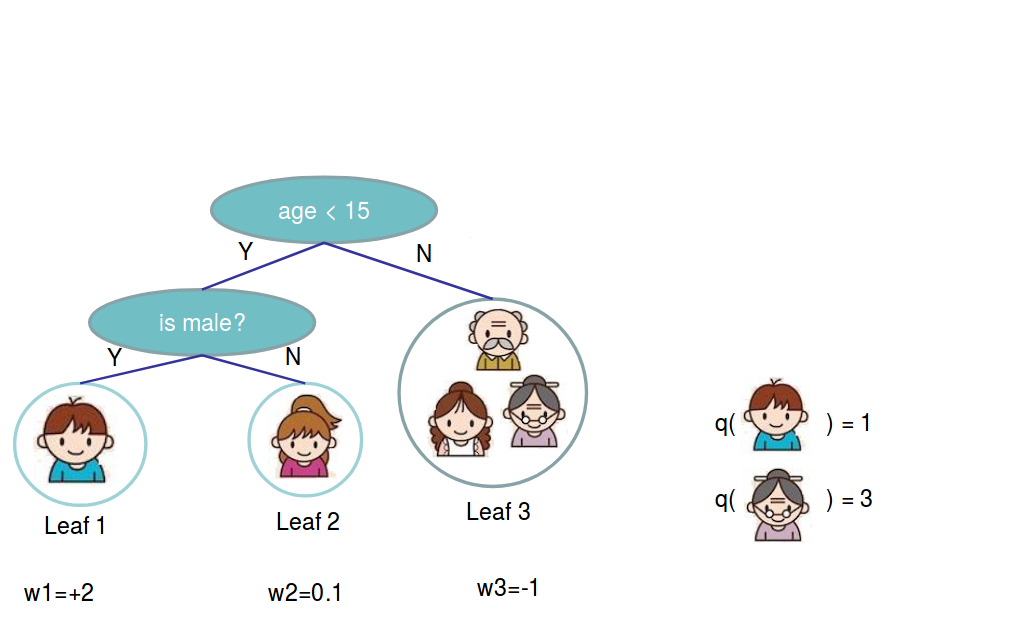
\includegraphics[scale=0.4]{Chapter2/Figs/refine-definition-tree.png}
    \caption{Ví dụ về cây theo cách định nghĩa mới}
    \label{fig:my_label2}
\end{figure}

Trong một số công cụ nổi tiếng như XGBoost\cite{4}, hàm regularization được định nghĩa như sau:

\begin{equation}
    \Omega(f) = \gamma T + \frac{1}{2}\lambda \sum_{j=1}^T w_j^2
\end{equation}

Như vậy, sau khi tái định nghĩa cây, hàm mục tiêu tại cây thứ $t$ được tính bởi: 
\begin{equation}
    \begin{split}Obj^{(t)} &\approx \sum_{i=1}^n [g_i w_{q(x_i)} + \frac{1}{2} h_i w_{q(x_i)}^2] + \gamma T + \frac{1}{2}\lambda \sum_{j=1}^T w_j^2\\
&= \sum^T_{j=1} [(\sum_{i\in I_j} g_i) w_j + \frac{1}{2} (\sum_{i\in I_j} h_i + \lambda) w_j^2 ] + \gamma T
\end{split}
\end{equation}

với $I_j = \{i|q(x_i)=j\}$ là tập hợp các chỉ số của các data point được gán cho lá thứ $j$. Đặt $G_j = \sum_{i\in I_j} g_i$ và $H_j = \sum_{i\in I_j} h_i$. (2.16) trở thành:

\begin{equation}
    \text{Obj}^{(t)} = \sum^T_{j=1} [G_jw_j + \frac{1}{2} (H_j+\lambda) w_j^2] +\gamma T
\end{equation}

% Xét hàm bình phương đơn biến:
% \begin{equation}
%   \begin{split}
%         \text{argmin}_x & G(x) + \frac{1}{2} Hx^2 = -\frac{G}{H} & \text{min}_x & Gx + \frac{1}{2}Hx^2 = -\frac{1}{2}\frac{G^2}{H}
%   \end{split}
% \end{equation}

Theo phương trình (2.17), ta có $G_jw_j+\frac{1}{2}(H_j+\lambda)w_j^2$ là một hàm bậc 2 đơn biến nên $w_j$ tốt nhất với các $q(x)$ cho trước và $\obj$ nhỏ nhất thu được là:
\begin{equation}
    \begin{split}w_j^\ast = -\frac{G_j}{H_j+\lambda}\\
\text{obj}^\ast = -\frac{1}{2} \sum_{j=1}^T \frac{G_j^2}{H_j+\lambda} + \gamma T
\end{split}
\end{equation}

\begin{figure}[H]
    \centering
    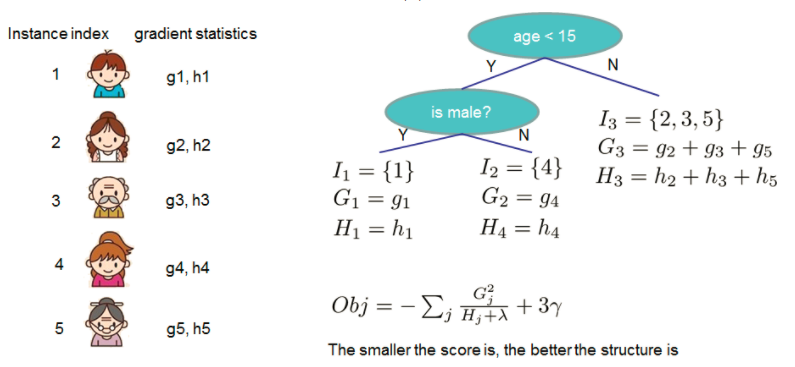
\includegraphics[scale=0.8]{Chapter2/Figs/objective-example.PNG}
    \caption{Ví dụ cách tính hàm mục tiêu}
    \label{fig:my_label3}
\end{figure}

\subsection{Học cấu trúc cây}

Để tìm cây tốt nhất tại mỗi lần lặp, phương án lý tưởng là duyệt tất cả các cấu trúc cây có thể. Nhưng điều này là bất khả thi vì số lượng cây rất lớn. Để giải quyết vấn đề này, tại mỗi mức, cây sẽ được tối ưu. Việc phân cây được thực hiện dựa trên cách tính $Gain$ mà mỗi lần tách lá thu được:

\begin{equation}
Gain = \frac{1}{2} \left[\frac{G_L^2}{H_L+\lambda}+\frac{G_R^2}{H_R+\lambda}-\frac{(G_L+G_R)^2}{H_L+H_R+\lambda}\right] - \gamma
\end{equation}

Phương trình (2.19) bao gồm 4 thành phần: Điểm tại lá trái, điểm tại lá phải, điểm tại lá ban đầu và regularization khi thêm lá mới. Nếu gain nhỏ hơn $\gamma$, việc phân nhánh là không cần thiết. Cách làm này được gọi là phương pháp cắt tỉa trên các mô hình cây. Với các dữ liệu thực, phương án tìm kiếm tối ưu đó là sắp xếp các thuộc tính tăng dầnvà thực hiện tìm kiếm để quyết định giá trị nào là tốt nhất để phân tách. \\

\begin{algorithm}[H]
 \caption{Thuật toán Tree Boosting}
 \label{algo_2}
 \begin{algorithmic}[1]
 \renewcommand{\algorithmicrequire}{\textbf{Input:}}
 \renewcommand{\algorithmicensure}{\textbf{Output:}}
\REQUIRE Dataset $D$\\
        Hàm mất mát $L$\\
        Số lượng cây $M$ \\
        Số lượng lá $T$ \\
        Learning rate \eta \\
        
% \ENSURE  Optimal value of $\alpha$ and base classifiers $BC_k$ ($k=1,\ldots ,K$)
%  \textit{(Khởi tạo bộ phân loại cơ sở)}
\STATE Khởi tạo $\hat{f}^{(0)}(x) = \hat{f}_{0}(x) = \hat{\theta}_0 = argmin_\theta \sum_{i=1}^{n}L(y_i,\theta);$  
\FOR{$m = 1\ldots M$}
    \STATE $\hat{g}_m(x_i) = [\frac{\partial L(y_i, f(x_i))}{\partial f(x_i)}]_{f(x)=\hat{f}^{(m-1)}}$;
    \STATE $\hat{h}_m(x_i) = [\frac{\partial^2 L(y_i, f(x_i))}{\partial f(x_i)}]_{f(x)=\hat{f}^{(m-1)}}$;
    \STATE Xác định ${\{\hat{R}_{jm}}\}^T_{j=1}$  bằng cách tìm cách chia sao cho cực đại hóa\\
    $Gain = \frac{1}{2}[\frac{G^2_L}{H_L} + \frac{G^2_R}{H_R} - \frac{G^2_{jm}}{H_{jm}}]$;
    \STATE Xác định trọng số lá $\{{\hat{w}_{jm}}\}_{j=1}^T$ cho cấu trúc học được bằng cách\\
    $\hat{w}_{jm}^T = -\frac{G_{jm}}{H_{jm}}$
    \STATE $\hat{f}_m(x) = \eta \sum_{j=1}^{T}\hat{w}_{jm}I(x \in \hat{R}_{jm})$;
    \STATE $\hat{f}^{(m)}(x) = \hat{f}^{(m-1)}(x) + \hat{f}_m(x)$;
\ENDFOR

\ENSURE  $\hat{f}(x) \equiv \hat{f}^{(M)}(x) = \sum_{m=0}^{M}\hat{f}_m(x)$
\end{algorithmic} 
\end{algorithm}

\subsection{Xử lý dữ liệu thiếu}

Nhiều giải thuật gặp vấn đề khi xử lý dữ liệu thiếu. Thường những điểm dữ liệu (data point) bị thiếu dữ liệu sẽ bị bỏ qua hoặc sẽ được tìm cách thêm giá trị tại bước tiền xử lý dữ liệu. \\
% CART xử lý các giá trị còn thiếu bằng cách sử dụng các biến được gọi là biến thay thế. Đối với mỗi dự đoán, chỉ sử dụng các quan sát mà dự báo đó không bị mất khi tìm kiếm cách phân tách. Khi một cách tách được chọn, nó sẽ tạo ra một danh sách các yếu tố dự đoán và điểm phân tách. Chúng được chọn để bắt chước tốt nhất việc tách các dữ liệu huấn luyện được thực hiện bởi phân tách chính.\\
Boosted Tree xử lý dữ liệu thiếu bằng cách học các hướng mặc định (default directions). Tại mỗi nút, sẽ có 2 hướng, trái hoặc phải. Trong quá trình dự đoàn, khi gặp dữ liệu bị thiếu, hướng mặc định sẽ được chọn. Khi gặp thiếu dữ liệu trong quá trình huấn luyện, hướng mặc định sẽ được học theo hướng làm tối thiểu hóa hàm mục tiêu. \cite{missing}

